\chapter{Introductie in de Arduino omgeving (week 1 en 2).}
\label{chap:intr}

Hierbij wordt er van uitgegaan dat een werkende Arduino omgeving aanwezig is en het voorbeeld programmaatje \texttt{\textbf{blink}} al een keer gerund heeft.

Als eerste volgt een korte uitleg aan de hand van het programma \texttt{\textbf{blink}} hoe een Arduino programma in elkaar zit en een korte beschrijving van een paar eigenschappen van de microbit pinnen. Verder zijn er een aantal opdrachten.


\section{ Hoe zit een Arduino programma in elkaar?}

We gaan even terug naar het \textbf{blinkdemo} voorbeeld uit de installatiehandleiding (zie listing \ref{lst:blink}).  Als het goed is heb je deze opgeslagen en kun je deze nu openen.

%\begin{lstlisting}[caption= Het programma blinkdemo.,label={lst:blink}]
	

%\end{lstlisting} 

\begin{lstlisting}[caption= Het programma blinkdemo,label={lst:blink},firstnumber=15]		
	
const int COL1 = 4;   // Colom #1 control, deze moet 0 zijn
const int LED = 21;   //ROW1 is poort 21.Dit is de linker boven LED.


void setup() {
	Serial.begin(9600);
	Serial.println("microbit is ready voor de embedded programmeur!");
	
	// omdat de LEDs in een matrix staan moet zowel de plus als de min aangestuurd worden.
	//De stroom loopt immers van + naar -
	pinMode(COL1, OUTPUT); //kolom is de -
	digitalWrite(COL1, LOW);
	pinMode(LED, OUTPUT);  //rij is de +
	
}

void loop() {
	Serial.println("blink!");
	digitalWrite(LED, HIGH);
	delay(500);
	digitalWrite(LED, LOW);
	delay(500);
}
\end{lstlisting}

Arduino noemt een dergelijk programma een schets (of ‘sketch’). 
Hierin zijn twee functieblokken herkenbaar: \texttt{{\textcolor{arduinoBlue}{void}} \textcolor{arduinoGreen}{setup}(){} en  \textcolor{arduinoBlue}{void} \textcolor{arduinoGreen}{loop}(){}}

Wat in het setup blok tussen de accolades {} staat, wordt éénmalig tijdens het opstarten uitgevoerd.

Als het setup blok klaar is, wordt het loop blok gestart. De code in het loop blok wordt continue herhaald, in principe duizenden keren per seconde. Het programma eindigt dus nooit!

Deze structuur (een opstartblok en een blok dat herhaald wordt) geldt voor alle type microcontrollers!

Aan het begin van de schets, vóór de \texttt{\textit{ \textcolor{arduinoBlue}{void} \textcolor{arduinoGreen}{setup}()}}, is plek voor het declareren van globale variabelen, deze variabelen kun je overal in het programma gebruiken, zowel in de setup als in de loop.

\colorbox{blue!15}{
	\begin{minipage}{\textwidth}
		Arduino gebruikt \textbf{kleuren} om \textcolor{BurntOrange}{functies} of \textcolor{BlueGreen}{uitdrukkingen} aan te geven. Als je wilt weten wat een dergelijk woord betekent of hoe je het gebruikt, klik dan in de Arduino IDE op het woord en druk 
		\colorbox{mygray}{\textbf{Ctrl + Shift + F}}
		
		Probeer dit uit: Selecteer in Arduino de tekens // en druk \colorbox{mygray}{\textbf{Ctrl + Shift + F}}.

	\end{minipage}
}

De \textcolor{BurntOrange}{oranje gekleurde functies} zijn geen deel van de taal C maar zijn gemaakt door Arduino en zijn gedefinieerd in Arduino libraries die standaard geïnstalleerd zijn. Deze functies maken het leven een stuk makkelijker! Ze vervangen een heleboel moeilijk leesbare C code.



\subsection{Code wijzigen.}

Wijzig in de schets de eerste \textcolor{BurntOrange}{delay}(500) naar \textcolor{BurntOrange}{delay}(100).


Klik op \img{figuren/ardIcUpl.png} of druk \colorbox{mygray}{\textbf{Ctrl + U}} om het programma te compileren en naar de Microbit te sturen.
Je ziet nu dat de ‘aan’ tijd korter is.

\subsubsection{Uitleg: Gebruik van de seriële poort}

In dit voorbeeld wordt de seriële poort gebruikt.

Je kunt de seriële poort gebruiken om te ‘debuggen’, oftewel controleren of je programma doet wat je er van verwacht. In The Challenge kun je het gebruiken om sensordata naar je PC te sturen.

Open de seriële monitor(Tools$\rightarrow$Serial Monitor) of (druk \colorbox{mygray}{\textbf{Ctrl + Shift + M}}) of klik op \img{figuren/ardIcMo.png}

Het programma drukt telkens ‘blink!’ af.\\ 
Zet “Show Timestamp” aan om de regels van elkaar te kunnen onderscheiden.\\ 
Zorg dat de ingestelde snelheid overeen komt met de instelling \textcolor{BurntOrange}{Serial.begin}(9600) in  \textcolor{OliveGreen}{setup}(). 
\begin{figure}[h!]
	\captionsetup{justification=centering}
	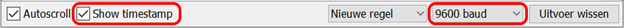
\includegraphics[width=0.99 \linewidth]{figuren/ardSerIns}
	\centering
	\caption{Instellingen van de seriële monitor.}
	\label{fig:arSeIn}
\end{figure}
De instellingen van de monitor kan gedaan worden in de statusbalk, zoals te zien is in figuur \ref{fig:arSeIn}.
Vaak wordt 9600 Baud (bits per seconde) gebruikt. Dit is gedaan omdat hiermee de data praktisch altijd stabiel verzonden wordt.

\subsection{Commando's verklaren.}

Geef in je eigen woorden weer wat de volgende commando’s doen (zoek uit via  \colorbox{mygray}{\textbf{Ctrl + Shift + F}})
\textcolor{BurntOrange}{pinMode}(LED, \textcolor{BlueGreen}{OUTPUT});\\
\vspace{1cm}
\hrule
~\\    
%\hrule
\vspace{1cm}
\textcolor{BurntOrange}{digitalWrite}(LED, \textcolor{BlueGreen}{LOW});\\
\vspace{1cm}
\hrule
~\\    
%\hrule
\vspace{0.8cm}
\textcolor{BurntOrange}{delay}(500);
 \vspace{1cm}
 \hrule
 ~\\    
 Wat denk je dat het grootste nadeel van \textcolor{BurntOrange}{delay}();  is?
 \vspace{1cm}
 \hrule
 
 \subsection{Dimmen van een led}
 
 We hebben al gezien dat je een pin als uitgang in kunt stellen en deze aan en uit kunt zetten.
 
 We gaan dezelfde pin nu op een andere manier gebruiken. We gaan de LED nu geleidelijk feller en minder fel laten branden, het Engelse werkwoord hiervoor is ‘to fade’. 
  \begin{enumerate}
 	\item  We gaan hierbij uit van de code uit de blinkdemo van listing \ref{lst:blink}.  Het knipperen van de LED wordt
 	in de \textcolor{arduinoGreen}{loop} gedaan, zoals in listing \ref{lst:blinkAfk} te zien is.
% 	\begin{lstlisting}[style=myArduino, caption= Het knipperen van de LED.,label={lst:blinkAfk},firstnumber=15]
  	\begin{lstlisting}[caption= Het knipperen van de LED.,label={lst:blinkAfk},firstnumber=15]		
 		void loop() {
 			
 			digitalWrite(LED, HIGH);
 			delay(500);
 			digitalWrite(LED, LOW);
 			delay(500);
 		}
 	\end{lstlisting} 
 	Hierbij wordt met het statement \textcolor{arduinoOrange}{digitalWrite}(LED, \textcolor{arduinoBlue}{HIGH}); de LED aangezet en met het statement \textcolor{arduinoOrange}{digitalWrite}(LED, \textcolor{arduinoBlue}{LOW}); de LED uitgezet.  In plaats van \textcolor{arduinoOrange}{digitalWrite} kan in sommige gevallen ook \textcolor{arduinoOrange}{analogWrite} gebruikt worden. Hiermee kan opgegeven worden hoeveel licht de LED geeft.
 	
 	Sla de blink op onder een andere naam, bijvoorbeeld Microbit-Fade. Verander de statement  \textcolor{arduinoOrange}{digitalWrite}(LED, \textcolor{arduinoBlue}{HIGH}); in \textcolor{arduinoOrange}{analogWrite}(LED, 10);
 	Klik vervolgens op \img{figuren/ardIcUpl.png} of druk \colorbox{mygray}{\textbf{Ctrl + U}} om het programma te compileren en naar de Microbit te sturen. Verklaar wat er gebeurd.
 	
 	Verander de 10 in een ander getal b.v. 70 en verklaar wat er gebeurd. De maximale waarde waarop de LED ingesteld kan worden is 255. Dit heeft te maken met het feit dat de waarde maar 8 bits groot is en 2$^{8}$ - 1 = 255.
 	%en het ingebouwde voorbeeld Fade van Arduino: Open Bestand $\rightarrow$ Voorbeelden $\rightarrow$ 01.Basics $\rightarrow$ Fade
 
 	\item  Pas het programma verder aan, zodat de LED steeds meer licht gaat geven. Indien de hoeveelheid licht die de LED geeft maximaal is, gaat de LED weer minder licht geven totdat de LED geen licht meer geeft, hierna gaat de LED weer meer licht geven, enz. Zoals weergegeven in het volgende filmpje\\  
 	\href{https://www.youtube.com/watch?v=J-VdHiCPVbQ/fade.mp4}{https://www.youtube.com/watch?v=J-VdHiCPVbQ/fade.mp4} te zien is.\\
 	\textbf{Lever deze opgave in op blackboard.}
   
  \end{enumerate}
 
 
 
\begin{comment}



 Gebruik de mogelijkheden van Arduino (en niet Google) om onderstaande vragen te beantwoorden, denk aan \colorbox{mygray}{\textbf{Ctrl + Shift + F}} en de commentaren die al in de code staan:
 Welke regel (welk commando) zorgt voor dit Fade effect? 


 \vspace{1cm}
 \hrule
 \vspace{1cm}
 Het mechanisme dat hier gebruikt wordt heet PWM. Waar staat de afkorting voor en wat doet het?
 \vspace{1cm}
 \hrule
 ~\\    
 \hrule
 \vspace{0.5cm}
\end{comment}
 Het mechanisme dat hier gebruikt wordt om de LED te dimmen heet PWM.\\
{ \texttt{\textit{Met PWM kun je niet alleen een led minder fel laten branden, maar zo kun je ook de snelheid van een motor regelen. De piepjes die je hoort bij een optrekkende tram of trein worden veroorzaakt door PWM aansturing.}}}
% \end{comment}
 
 \subsection{Het ontvangen van informatie vanaf de arduino-monitor en de beide knoppen.}
 
 Behalve dat de microbit data naar de monitor kan verzenden, kan deze ook data van de  monitor lezen.
 Dit kan gedaan worden door de data in het bovenste vierkant (zoals in figuur \ref{fig:ardMonRd} wordt weergegeven) in te typen en vervolgens op \textbf{Send} te klikken.
 \begin{figure}[h!]
 	\captionsetup{justification=centering}
 	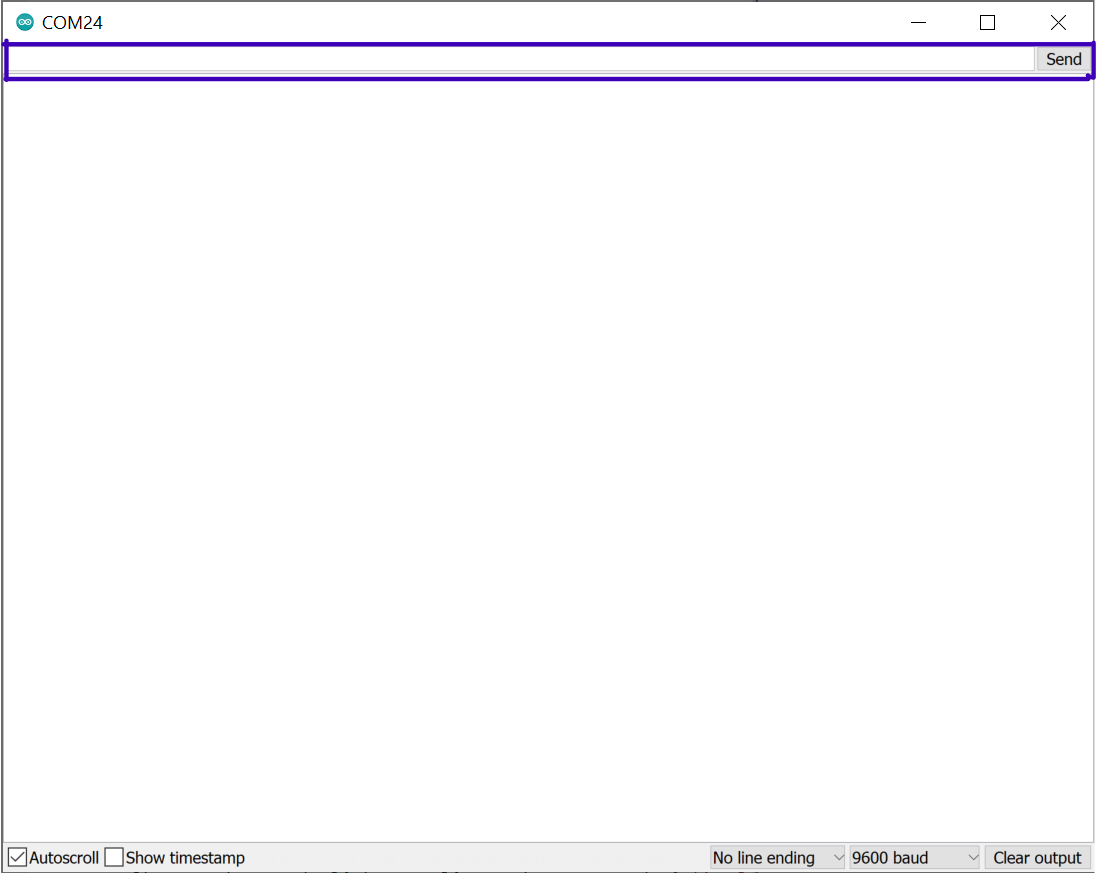
\includegraphics[width=0.6 \linewidth]{figuren/arduinoMonRd}
 	\centering
 	\caption{Inputveld van de arduino monitor.}
 	\label{fig:ardMonRd}
 \end{figure}
Om in je programma de data te lezen, zal eerst gecheckt moeten worden of er al data via de seriële poort binnen gekomen is, dit kan gedaan worden met het statement:  \texttt{if(\textcolor{BurntOrange}{Serial.available}() \textgreater 0) \{ \}} daarna kan de data pas gelezen worden. 
Dit wordt gedaan met het statement:   \texttt{int getal=\textcolor{BurntOrange}{ Serial.read}();}, zoals te zien is in listing \ref{lst:serInp}.

%\begin{lstlisting}[style=myArduino,numbers=none ,caption= inlezen via de seriele poort.,label={lst:serInp}]
\begin{lstlisting}[numbers=none ,caption= inlezen via de seriele poort.,label={lst:serInp}]	
int getal=0;

void setup() {  
	Serial.begin(9600);
	Serial.println("Hoi embedded programmeurs!");
	
}

void loop(){
	if (Serial.available() > 0) {  //is er een character ingevoerd?
		getal= Serial.read();
		Serial.println(getal);
	}
}
\end{lstlisting} 
 Opdracht:
 
  \begin{enumerate}
 	\item Voer de code van Listing \ref{lst:serInp} uit en type in het invoerveld van de monitor de cijfers 012345 in, gevolgd door een enter.
 	Als het goed is verschijnt Figuur \ref{lst:serInp}
 
 \begin{figure}[h!]
 	\captionsetup{justification=centering}
 	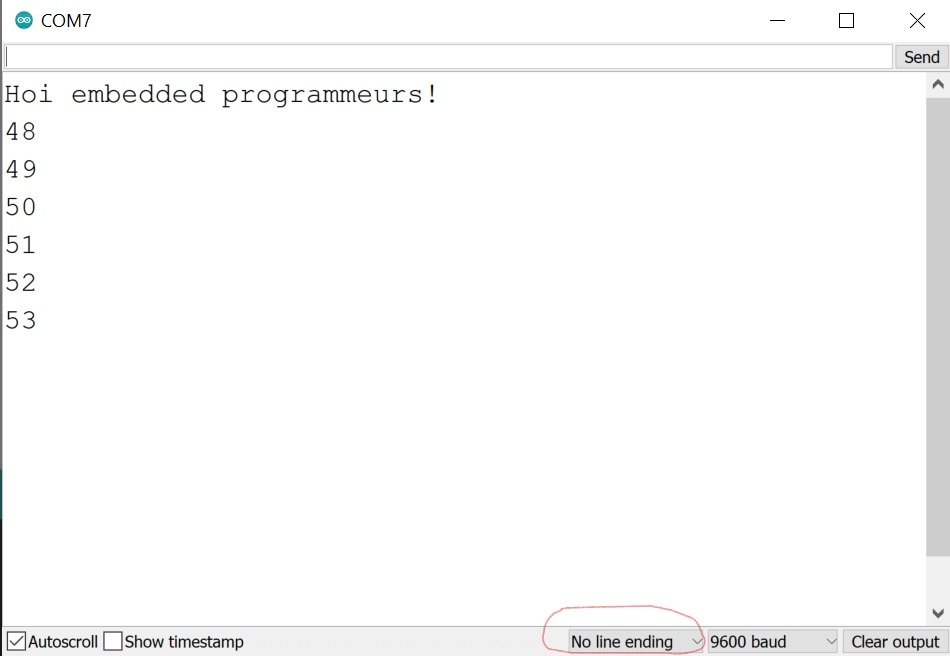
\includegraphics[width=0.6 \linewidth]{figuren/ardMonChar.jpg}
 	\centering
	\caption{Uitvoering van listing \ref{lst:serInp}}
 		\label{fig:ardMonChr}
 \end{figure}
Wat opvalt is dat in plaats van het getal 012345 de getallen 48, 49, 50, 51, 52 en 53 worden uitgeprint. Dit heeft te maken dat het statement 
\texttt{int getal=\textcolor{BurntOrange}{ Serial.read}();} een character inleest, waarbij elke character een waarde heeft volgens de \href{https://nl.wikipedia.org/wiki/ASCII_(tekenset)}{ASCII} tabel.\\
Let op: Indien de monitor anders ingesteld staat dan "\texttt{\textit{No line ending}}", worden de onzichtbare characters (line feed en/of carriage return ) getoond. 
\item Pas het programma van listing 1 zodanig aan, zodat na invoering van je studentnummer en gebruik van het statement \texttt{int getal=\textcolor{BurntOrange}{ Serial.read}();} ook daadwerkelijk je studentnummer als een integer uitprint kan worden. 
 \begin{figure}[h!]
	\captionsetup{justification=centering}
	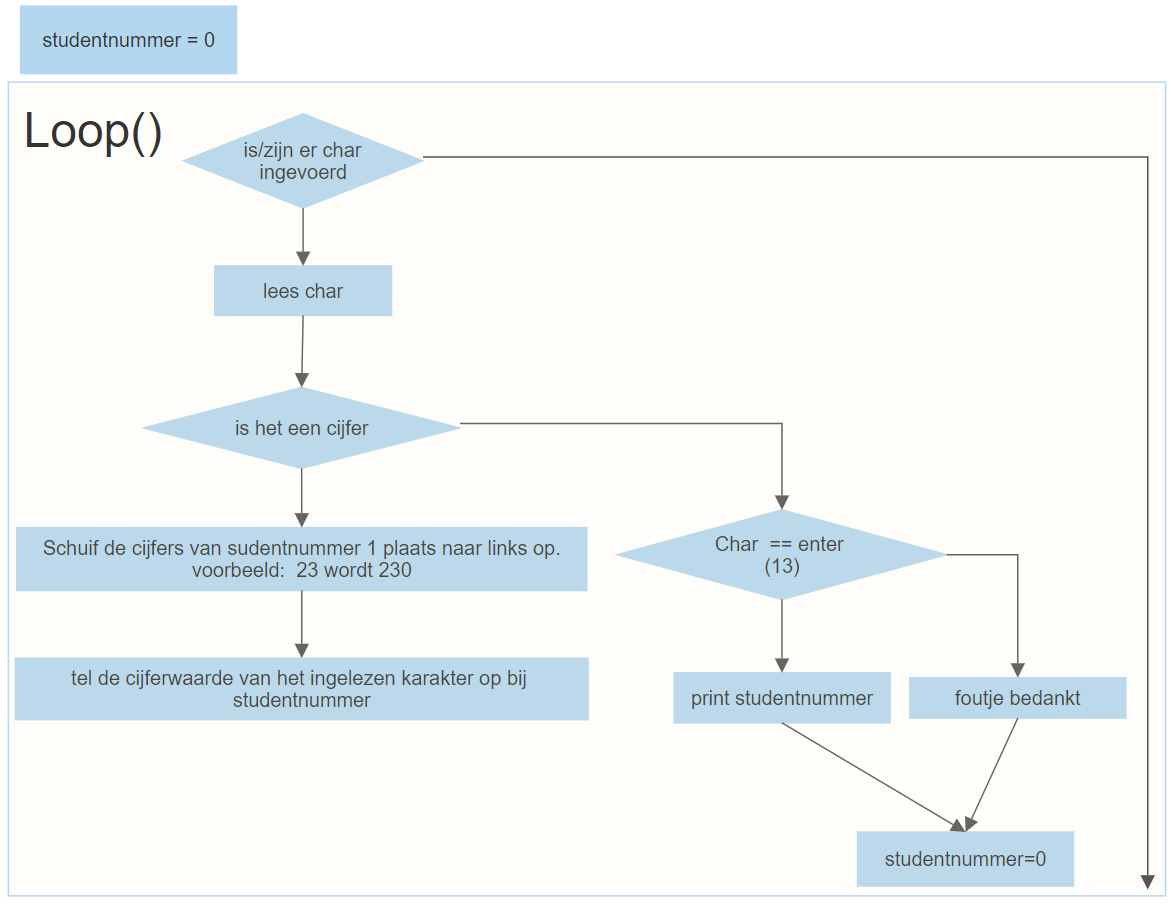
\includegraphics[width=0.8 \linewidth]{figuren/nummerloop}
	\centering
	\caption{diagram om  losse cijfers om te zetten naar een int. }
	\label{fig:progFig}
\end{figure}
Een schematische weergave van de oplossing, wordt in Figuur \ref{fig:progFig} weergegeven.
\small{Tip: kijk naar de sheets over het \textbf{decimale talstelsel met grondtal 10}}.\\
\textbf{Lever deze opgave in op blackboard.}
\end{enumerate}

\section{De (externe) pinnen van de microbit}
 
De Microbit heeft 21 pinnen (aansluitingen) die voor allerlei toepassingen bruikbaar zijn. In figuur \ref{fig:ardPinB} zijn de externe aansluitingen van de microbit te zien. 
\begin{figure}[h!]
	\captionsetup{justification=centering}
	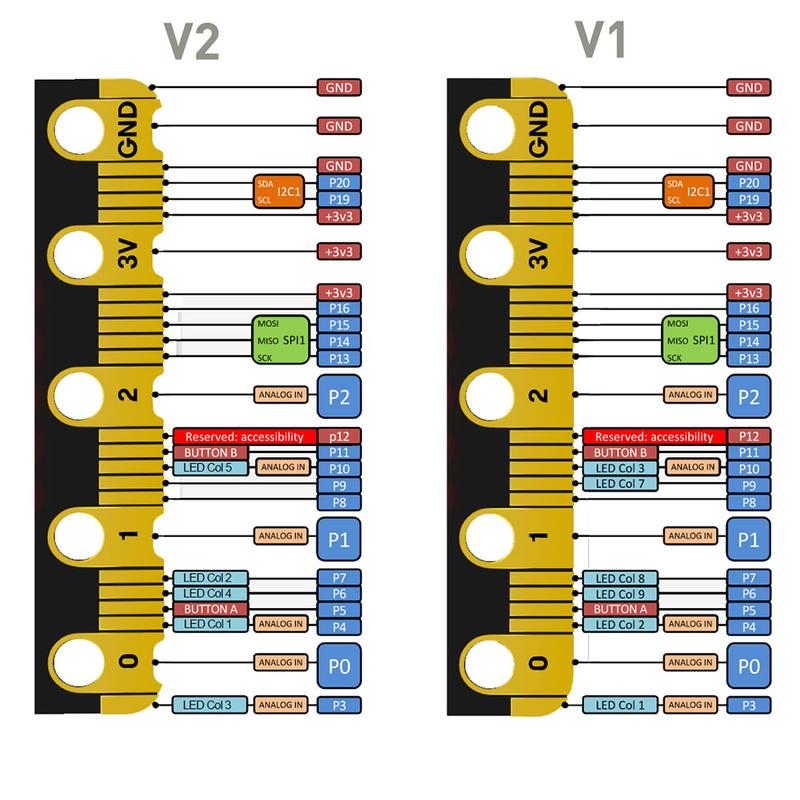
\includegraphics[width=0.6 \linewidth]{figuren/microbitCon.jpg}
	\centering
	\caption{Pinlayout van de microbit.}
	\label{fig:ardPinB}
\end{figure}
Hierbij wordt aangegeven welke onderdelen van de microbit ook extern zijn te gebruiken. Bij de pinnen waarbij \fcolorbox{black}{Apricot}{ANALOG IN} staat, kan een externe analoge signaal van b.v. een externe sensor aangesloten worden. De pinnen genaamd \fcolorbox{black}{NavyBlue}{\textcolor{White}{P..}} zijn de pinnummers. In de Arduino IDE kan je die P weglaten en hoef je alleen het nummer op te geven, 0 t/m 20. Uitgebreidere informatie over de pinnen is te vinden op de website \href{https://tech.microbit.org/hardware/edgeconnector/}{tech.microbit.org/hardware/edgeconnector/}.\\
%\newpage

\subsection{Het lezen van externe signalen met de microbit.}

Stel op PIN P0 willen we een externe analoge sensor aansluiten. Voor de spanningswaarde die de sensor levert willen we een digitale waarde weten. 
Dit kan in de Arduino omgeving gedaan worden me het statement:\\

int sensorwaarde = \textcolor{arduinoOrange}{analogRead}(A0);

\begin{enumerate}
%	\item  Open \textbf{Bestand $\rightarrow$ Voorbeelden $\rightarrow$ 01.Basics $\rightarrow$ AnalogReadSerial}.
\item In programma listing \ref{lst:analogInp} wordt het analoge signaal van de externe PIN P0 gelezen.
%\begin{lstlisting}[style=myArduino,numbers=none ,caption= inlezen via een analoog signaal.,label={lst:analogInp}]
\begin{lstlisting}[numbers=none ,caption= inlezen via een analoog signaal.,label={lst:analogInp}]
	void setup() {  
		pinMode(0, INPUT); 
		Serial.begin(9600);
		Serial.println("Hoi embedded programmeurs!");
	}
	
	void loop(){
          // lees de analoge waarde op pin 0:
        int sensorValue = analogRead(A0);
        
        // print de ingelezen analoge waarde
        Serial.println(sensorValue);
        delay(100);        // delay 
	}

\end{lstlisting}
\begin{enumerate}
	\item  Maak een nieuw Arduino sketch aan en zet listing \ref{lst:analogInp} erin, Klik vervolgens op \img{figuren/ardIcUpl.png} of druk \colorbox{mygray}{\textbf{Ctrl + U}} om het programma te compileren en naar de Microbit te sturen. 
\item Zoek PIN 0 in Figuur \ref{fig:ardPinB}.
\item Leg je Microbit op tafel, raak hem niet aan. 
\item De Arduino omgeving heeft behalve een Seriële monitor ook een Seriële Plotter. Helaas kan maar één van beide monitor of plotter gebruikt worden. 
Indien de Seriële monitor open is, sluit deze dan en open de Seriële Plotter ( Tools $\rightarrow$ Serial Plotter of \colorbox{mygray}{\textbf{Ctrl + shift + L}}).
Raak met je vinger het gouden vlakje van pin 0 aan en kijk in de Seriële Plotter wat er gebeurt.
\item Tussen welke waardes op de linker as liggen de meetwaardes? \hrulefill \\	
 \footnotesize{\texttt{\textit{(Bij mij kwam deze uit tussen de 1000 zonder aanraken en de 750 )}} }
	
\end{enumerate}


\item Verander he statement  \textcolor{arduinoOrange}{analogRead}(A0); in \textcolor{arduinoOrange}{digitalRead}(A0); Klik vervolgens op \img{figuren/ardIcUpl.png} of druk \colorbox{mygray}{\textbf{Ctrl + U}} om het programma te compileren en naar de Microbit te sturen. Raak met je vinger het gouden vlakje van pin 0 aan en kijk in de Seriële Plotter wat er gebeurt. 

\item Bij het inlezen van een digitaal signaal is het niet wenselijk dat bij het aanraken van een draadje of een gouden vlakje de ingangswaarde instabiel wordt. Om dit te voorkomen kan bij Arduino de  \textcolor{arduinoBlue}{INPUT\_PULLUP} aangezet worden. Dit wordt gedaan met het statement: \textcolor{arduinoOrange}{pinMode}(0,\textcolor{arduinoBlue}{INPUT\_PULLUP}); 

\begin{minipage}{\linewidth}
\begin{wrapfigure}[25]{r}{0.54\textwidth}
	\vspace{-15pt}
	\begin{center}
		\centering
		\captionsetup{justification=centering}
		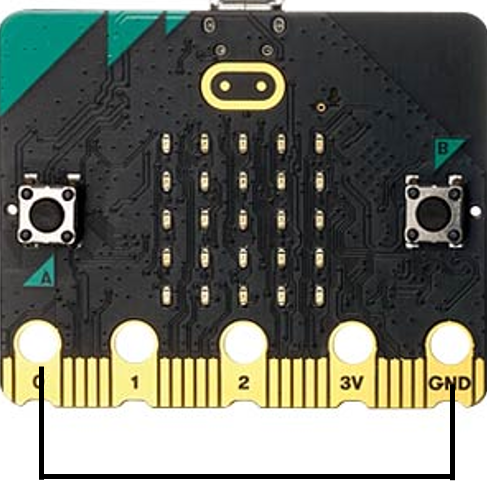
\includegraphics[width=0.32\textwidth]{figuren/microBitDraad}
	\end{center}
%	\vspace{-14pt}
	\caption{Input verbonden met de GND .}
	\label{fig:micrDraad}
\end{wrapfigure}
Zet de \textcolor{arduinoBlue}{INPUT\_PULLUP} aan door het statement 
\textcolor{arduinoOrange}{pinMode}(0,\textcolor{arduinoBlue}{INPUT\_PULLUP});  
te plaatsen in de \textcolor{arduinoGreen}{setup} en bekijk wat het resultaat is bij het inlezen van de digitale en analoge waarden. Indien je een draadje bij de hand heb, verbindt de GND met PIN 0, zoals te zien is in figuur \ref{fig:micrDraad}, het gevolg van de PULL\_UP zal zijn dat alleen nog de waarde 0 ingelezen wordt indien de pin ook daadwerkelijk verbonden wordt met de GND.
\end{minipage}



\begin{comment}
Zet de \textcolor{arduinoBlue}{INPUT\_PULLUP}  aan door het statement  \textcolor{arduinoOrange}{pinMode}(0,\textcolor{arduinoBlue}{INPUT\_PULLUP});  
te plaatsen in de \textcolor{arduinoGreen}{setup} en bekijk wat het resultaat is bij het inlezen van de digitale en analoge waarden.
\end{comment}
\end{enumerate}
\begin{comment}
Wat zie je gebeuren? 
\vspace{1cm}
\hrule
\vspace{0.8cm}
Tussen welke waardes op de linker as liggen de meetwaardes? \hrulefill

Hoeveel bits zijn nodig om dit getal (de hoogste waarde) weer te geven?  \hrulefill

Voeg nu deze regel toe in het \textcolor{OliveGreen}{setup}() deel:

\hspace{1cm}
\textcolor{BurntOrange}{pinMode}(0,\textcolor{BlueGreen}{INPUT\_PULLUP});\\

Sla je programma op met \colorbox{mygray}{\textbf{Ctrl + S}} en upload het programma met \colorbox{mygray}{\textbf{Ctrl + U}} , open de Seriële Plotter.

Wat zie je nu gebeuren?
\vspace{1cm}
\hrule
Tussen welke waardes op de linker as liggen de meetwaardes? \hrulefill
\end{comment}
%\newpage
\begin{minipage}{\linewidth}
\footnotesize{\texttt{\textit{Zoals je ziet is de ingang ongevoelig als je \textcolor{arduinoBlue}{INPUT\_PULLUP} aanzet. Je gebruikt \textcolor{arduinoBlue}{INPUT\_PULLUP} als je een ingang naar een stabiele ‘hoog’ toestand wilt hebben. Je gebruikt deze modus samen met digitalRead() als je een schakelaar wilt uitlezen. Als je de schakelaar indrukt wordt de pin laag.\\
De knopjes op de Microbit gebruiken een \textbf{externe} pull-up weerstand, met \textcolor{arduinoBlue}{INPUT\_PULLUP} zet je een pull-up weerstand in de microcontroller aan.\\ Kijk eens online voor meer uitleg over de principes van een  \href{https://www.freecodecamp.org/news/a-simple-explanation-of-pull-down-and-pull-up-resistors-660b308f116a/}{pull\_up weerstand}.\\ \\
Voor verdere uitleg zie \href{https://www.arduino.cc/en/Tutorial/DigitalPins}{www.arduino.cc/en/Tutorial/DigitalPins}
}}}
\end{minipage}
\normalsize
\subsection{Een denderende schakelaar.}

Behalve dat bij het inlezen van de waarde van een externe schakelaar regelmatig een pull\_up weerstand noodzakelijk is. 
Treedt er nog een ander probleem op, namelijk een schakelaar die dendert ook wel bouncing genaamd.

Indien een schakelaar wordt ingedrukt sluit deze bijna nooit in 1 keer, maar veert een aantal keren op en neer. Dit fenomeen wordt weergegeven in Figuur \ref{fig:swDend}, 
\begin{figure}[h!]
	\captionsetup{justification=centering}
	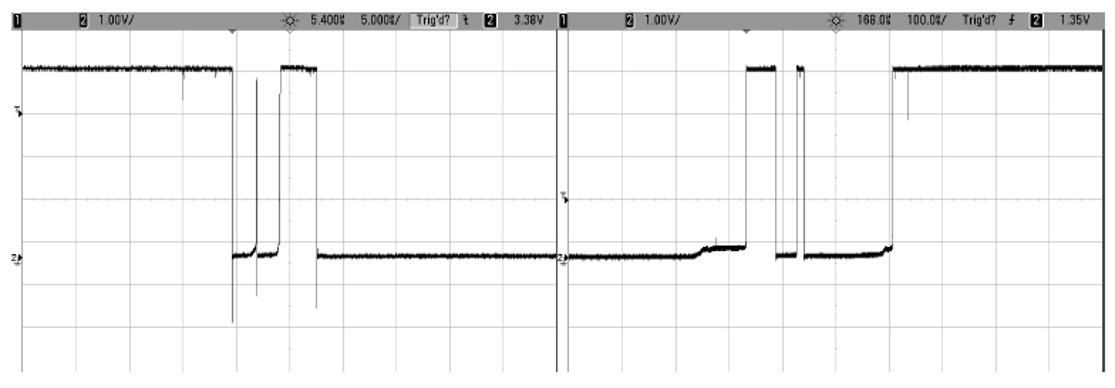
\includegraphics[width=0.6 \linewidth]{figuren/denderen}
	\centering
	\caption{Een denderende schakelaar\cite{williams2014make}.}
	\label{fig:swDend}
\end{figure}
waar te zien is dat bij het indrukken en loslaten van het knopje de schakelaar 'stuitert'. 
Één van de eenvoudigste manieren om dit op te lossen is door even te wachten (een paar milliseconden) en vervolgens te controleren of de knop nog steeds is ingedrukt. Dit wordt weergegeven in listing \ref{lst:denderBut}
%\begin{lstlisting}[style=myArduino, caption= Omgaan met een denderende schakelaar.,label={lst:denderBut}]
\newpage
\begin{lstlisting}[caption= Omgaan met een denderende schakelaar.,label={lst:denderBut}]
const int knopA = 5;     // Knop A is aangesloten op poortnummer 5
const int knopB = 11;    // Knop B is aangesloten op poortnummer 11

void setup() {  
	Serial.begin(9600);
	Serial.println("microbit is ready!");
	
	pinMode(knopA, INPUT);  
	pinMode(knopB, INPUT);   
}
boolean isKnopIngedrukt(int); //declaratie van de funcie

void loop(){
	
	if( isKnopIngedrukt(knopA) )
	Serial.println("A is ingedrukt");
	
	if( isKnopIngedrukt(knopB) )
	Serial.println("B is ingedrukt");       
	
	delay(10);
}

boolean isKnopIngedrukt( int knop) {
	if (! digitalRead(knop)) {  //Is de knop soms ingedrukt ?
		delay(2);      //wacht 2 milliseconde 
		if (! digitalRead(knop)) { //Is knop nog steeds ingedrukt
			return true;
		}
	}
	return false;
}
\end{lstlisting}

Hierbij wordt in de functie \texttt{\textit{\textcolor{arduinoBlue}{boolean} isKnopIngedrukt(\textcolor{arduinoBlue}{int});}} als eerste gekeken of de knop is ingedrukt, vervolgens wordt er 2 miliseconde gewacht, waarna opnieuw gekeken wordt of de knop is ingedrukt. Is dit zo dan wordt een \textcolor{arduinoBlue}{true} mee teruggegeven anders een \textcolor{arduinoBlue}{false}.

In listing \ref{lst:changeBut} is te zien dat er een detectie plaatsvindt wanneer de toestand van de schakelaar verandert.
\begin{lstlisting}[caption= Een toestandverandering van de schakelaar.,label={lst:changeBut}]

const int COL1 = 4; 
const int ROW1 = 21;
const int knopA = 5;     // Knop A is aangesloten op poortnummer 5
const int knopB = 11;    // Knop B is aangesloten op poortnummer 11

boolean isKnopIngedrukt(int);

int knopTeller = 0;  
boolean knopToestand = false;
boolean vorigeKnopToestand = false;
int ledStatus = LOW;

void setup() {  
	Serial.begin(9600);
	Serial.println("microbit is ready!");
	pinMode(COL1, OUTPUT);
	pinMode(ROW1, OUTPUT);
	pinMode(knopA, INPUT);  
	pinMode(knopB, INPUT);   
    digitalWrite(COL1, LOW);
}

void loop(){
	knopToestand = isKnopIngedrukt(knopA);
	if(knopToestand != vorigeKnopToestand)  //heeft er een verandering plaatsgevonden?
	if (knopToestand == true) {
		knopTeller++;
		ledStatus = !ledStatus;
		Serial.println(knopTeller);
	}
	delay(50);
	vorigeKnopToestand = knopToestand;
	digitalWrite(ROW1, ledStatus);
}

boolean isKnopIngedrukt( int knop) {
	if (! digitalRead(knop)) {  //Is de knop soms ingedrukt ?
		delay(2);      //wacht 2 milliseconde 
		if (! digitalRead(knop)) { //Is knop nog steeds ingedrukt
			return true;
		}
	}
	return false;
}

\end{lstlisting}

%Open Bestand $\rightarrow$ Voorbeelden $\rightarrow$ Microbit-HHS $\rightarrow$ 04B.StateChangeDetection en
Open het voorbeeldprogramma \texttt{\textit{veranderToestandDrukknop.ino}} (dit is listing \ref{lst:changeBut} )en upload het naar de Microbit.
Bestudeer de code en kijk hoe het programma werkt. Het is de bedoeling dat na elke druk op knopA de led aan of uit gaat (wisselt van toestand) en dat de teller steeds met 1 opgehoogd wordt. 
	\begin{enumerate}[label=(\Alph*)]

	\item In figuur \ref{fig:swToestand} wordt het signaal van de button weergegeven.
\begin{figure}[h!]
	\captionsetup{justification=centering}
	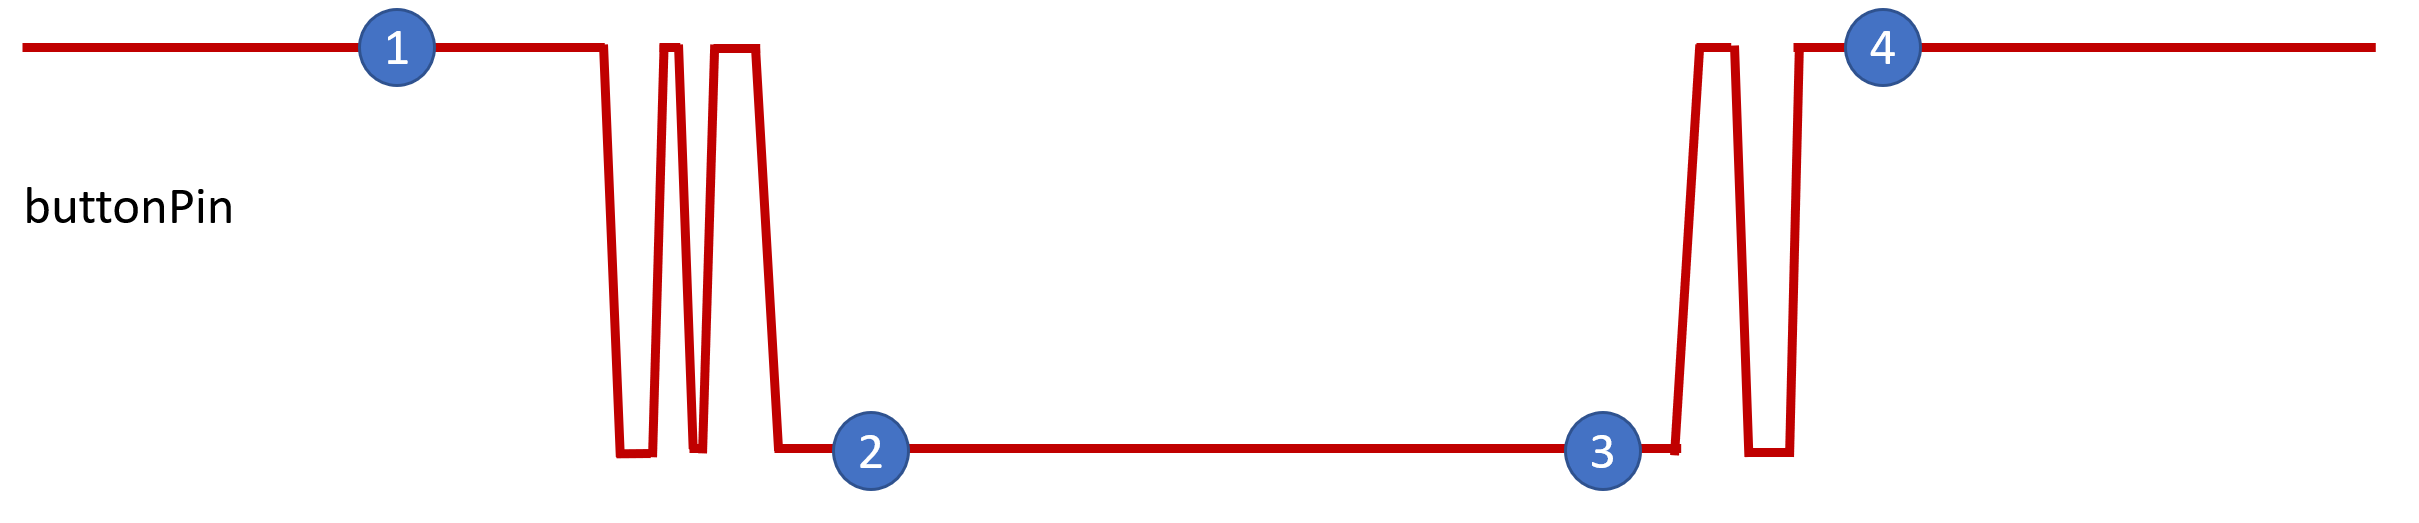
\includegraphics[width=0.8 \linewidth]{figuren/toestandButtonPin}
	\centering
	\caption{Weergaven van het signaal, indien de button wordt ingedrukt en weer wordt losgelaten.}
	\label{fig:swToestand}
\end{figure}
In welke toestand (1 t/m 4 )  bevindt zich de variabele \texttt{knopToestand} en \texttt{vorigeKnoptoestand} indien de toestand van de LED verandert en de teller met 1 verhoogd wordt?
\item Wat is het nut van het statement \textcolor{arduinoOrange}{delay}(50) op regel 31?\hrulefill
\item Wat is het resultaat indien de outputpin COL1 van listing \ref{lst:changeBut} op \textcolor{arduinoBlue}{HIGH} gezet wordt?	
\item Breid listing \ref{lst:changeBut} uit, zodat de teller met 1 verlaagd wordt indien met knopB een toestand verandering van 3 naar 4 plaatsvindt.\\
\textbf{Upload deze opgave op blackboard.}
	
\end{enumerate}

